\chapter{The GitHub Way}
This chapter describes GitHub in detail, outlining what it is, how it is used, what are some of its defining features, and why it might be used in education. GitHub exemplifies what we call `The GitHub Way': the way in which users of GitHub and similar platforms work and collaborate, where multiple contributors can edit, add to, and discuss work. This is an important distinction, as this work investigates how not just GitHub, but rather the activities that GitHub supports, can impact education. %as we feel it is not just GitHub itself that can impact education, but rather the activities that GitHub supports.

\section{What is GitHub?}
GitHub is web-based social code sharing service that utilizes the Git distributed version control system. It is a tool utilized by millions of developers all over the world to facilitate collaboration via the use of its awareness and transparency features, collaborative features such as pull requests, and version control. The tool is organized so that developers can create repositories containing code, which they can cultivate on their own or share with other developers who can, in turn, contribute to the code. Repositories can be public, which means that anybody can see them and pull their code, though the owner can decide who can and cannot make changes; or they can be private, making the repository viewable and editable only by those given collaborator status.

\section{Git: Distributed Version Control}
Git is the underlying version control system that GitHub utilizes. There's two very important aspects to Git: that work is distributed, and that work is handled by version control. To be distributed refers to the possibility of work being decentralized; instead of being forced to work in a repository where there is a central hub where everyone pushes code to, individual developers can create public `Clones' of that repository and `Push' to their respective clones before the original repository's maintainer or owner pulls in the work. This provides many opportunities for remixing and reusing code as well as creating a workflow in which multiple parties can do separate work at their own pace.

Version control means that developers can easily track changes to their code and that multiple developers can work on the same file, as combining changes requires a simple `Merge' process that Git handles. In this system, when a user makes changes to the project, they would `Commit' their changes, effectively saving a snapshot of the project as it is at that point of time. These commits, or snapshots, are saved in history, allowing developers to revert projects back in history as needed. The user can then push all of their changes to the server, meaning other collaborators can see these changes made. If a collaborator has made changes as well, these can be merged together to combine the different changes into the main code base.

\section{Branching \& Forking}
`Branching' and `Forking' provides two ways of diverging from the main code base. A user can make changes in a repository `Branch', which is a deviation of the code from the code base (the `trunk') and the changes remain a part of the main repository \footnote{\url{https://guides.github.com/introduction/flow/}}. When a user branches off the trunk, they can still monitor changes to the trunk despite working on a different branch of it.

`Forking', meanwhile, achieves a similar function of deviating from the code base. The main difference is that a fork is independent of the main code base, meaning a user won't be aware of the changes happening in the repository of the main code base unless they are explicitly watching the original repository \footnote{\url{https://help.github.com/articles/fork-a-repo/}}. When a user forks a repository, the repository, including all of its branches, are copied; on the other hand, if a repository is deleted, the fork still exists.

Generally, branching provides a good workflow for development teams, where collaborators need to be aware of all the changes made to each branch and the main code base. Meanwhile, forking tends to work for open-source projects where the repository owner does not want to manage user access to the repository and would want to keep collaborator changes independent until they are ready to be merged.

\section{Merging \& Pull Requests}
`Merging' is the mechanism for combining changes with each other or pulling changes in a branch or fork into the main code base. For example, a collaborator can branch or fork from the main code base and make changes to the code as they see fit, and it would remain on their branch or on their repository. In order to get the changes into the main code base, a person managing the repository, a maintainer, would have to merge the changes into it, combining whatever changes were made in the branch or fork with the code base as it is. In some cases such as when the same section of code is changed at the same time, this can result in what's called a merge conflict, which would require the user to manually pick and choose which of the changes or pieces of code they want to keep. These merge conflicts would be an issue in file types that aren't versioned by Git, such as PDF documents, as changes anywhere in the file in two different branches could create merge conflicts.

\begin{figure}[h!]
 \caption{An example of a Pull Request in AngularJS, a popular open-source repository.}
 \centering
   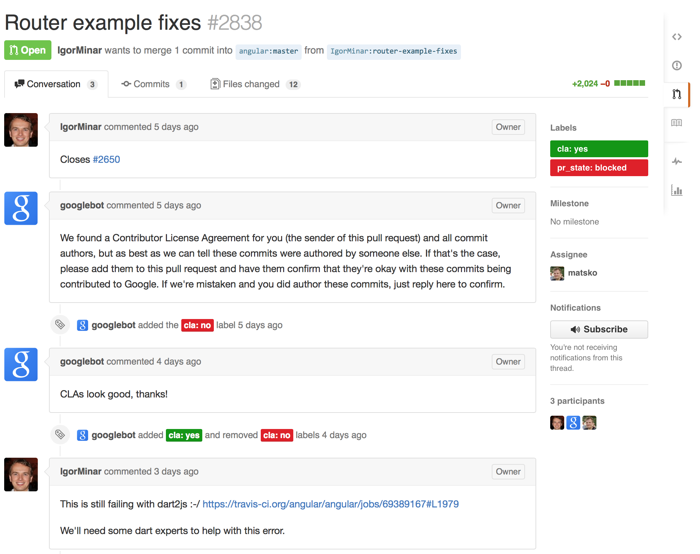
\includegraphics[width=0.8\textwidth]{pullRequests}
 \label{fig:pull_requests}
\end{figure}

`Pull Requests' (PRs) are a way of handling these merges. In a PR, the person making the changes in a branch or a fork will request to the code base maintainer to merge their code into the main trunk, otherwise known as the master branch. These PRs will be listed on GitHub in a separate tab, where collaborators can see each of the commits made, what files were changed, and the conversation surrounding the code, as seen on figure \ref{fig:pull_requests}. Collaborators can also make comments on PRs, typically when changes have to be made before a PR should be accepted or a `+1' if they think a PR is ready to be merged into the main code base.

\section{Issues \& Comments}
The `issues' feature on GitHub allows for discussion between collaborators. These issues can be tagged with any label the issue creator or editor wants, such as `Bug' or `Feature', and the issues list can be filtered to only see issues of a certain tag, or see only closed or open issues. Issues can be assigned to a user, letting others know who is in charge of that issue. As well, issues can be assigned to a `Milestone', a date set by a collaborator to have certain issues completed by. PRs are also automatically posted as an issue, which gets closed when that PR gets accepted or closed. Users can comment on issues, so the issues can be used as a hub for discussions. Users can also refer to issues in commit messages, thereby displaying it in the issue: for example, an issue, when fixed by a commit, could say \textit{``collaborator closed this in d2ad525 on Oct. 25, 2014.''}

Moreover, an important feature is in the flexibility afforded to users making comments. For example, users can mention others by referring to their username preceded by an `@' character, thereby sending them a notification and, in most cases, an email. This allows collaborators to directly refer to another when, for example, they'd like to ask someone to make a specific change to an issue or PR. Users can also comment on more specific artifacts, such as pull requests, commits, or individual lines of code. This gives the user flexibility in being able to discuss various aspects of a project with another collaborator; for example, when a specific line of code is difficult to understand or causes a bug, that line of code can be distinguished as the issue.

\section{Openness \& Transparency}
GitHub's openness and transparency features allows groups to facilitate both direct and indirect collaboration, allowing users to have a full view of activities occurring in the project. For example, users can look at the commit history to see exactly what the other collaborators are working on and changing, as they are able to see specific changes on specific commits. This history is useful, compounded by the use of the `blame' feature, in which a user can see exactly who made a specific change or line of code. %why is this useful

\begin{figure}[h!]
 \caption{An example what a user would see in the News Feed.}
 \centering
   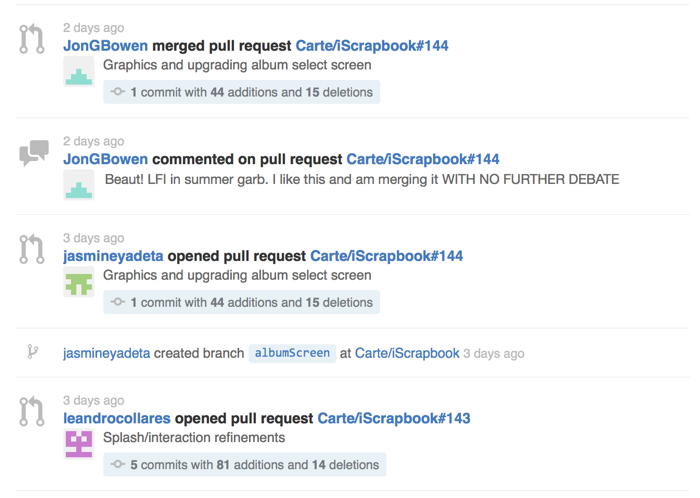
\includegraphics[width=0.8\textwidth]{newsFeed}
 \label{fig:news_feed}
\end{figure}

Upon logging into GitHub, the first screen the use will see is their News Feed \footnote{\url{https://help.github.com/articles/news-feed/}}. This News Feed includes all the activity on all the repositories that the user is involved in or is `Watching', a feature described below. Any comments, pushes to code, pull requests, or created issues appear in this News Feed, allowing the user to be aware of the events happening in their repositories. Figure \ref{fig:news_feed} is an example, where the user becomes aware of the activities happening in the repository.

GitHub also includes the `Watch' feature, which has three options. If a user chooses to be `Watching' a repository, they will get notifications from the activity in that repository, including changes to the code base, new pull requests, new issues, and comments on PRs, issues, commits, or code. These notifications appear in three potential places---the user's news feed, as a notification in their notifications list, and as an email. Alternatively, a user can choose `Not Watching', meaning they will only be notified if they are specifically mentioned in a comment or commit, or in comment threads that they have participated in. Finally, they can choose `Ignoring' on a repository, which will result in not receiving any notifications for that repository in any capacity.

The last important feature that promotes openness and transparency is the activity monitor on a repository. On the activity monitor, a user can look at who has contributed to the repository---for example, graphs of number of commits from each person or lines of code added by each person. Beyond that, numerous features allow a user to get a more wholistic picture of the activity on the repository, such as what time commits are normally made on each day, or how each branch is handled in comparison to the master branch, or how many times the repository has been visited. Overall, this feature allows a user to see and compare activity of all collaborators.

\section{Why GitHub for Education?}
Up until recently, GitHub has focused on code and project management for software development; it is now being extended to other domains that involve collaborative work, such as education \cite{Griffin:2013:GCJ:2458539.2458551}. However, the use of GitHub in this different context might require instructors to change their teaching technique or curriculum, or require GitHub to be repurposed to better accommodate for teaching activities. Jim Baker, a senior developer and University of Colorado Computer Science lecturer, shared his experiences with GitHub: \begin{quote}\textit{``We had a great experience using GitHub to support a collaborative workflow for the 70+ students in each of the 2 semesters of my CS course.''}\end{quote} He elaborated: \begin{quote}\textit{``Pull requests (PR) are the heart of the GitHub workflow, and we took advantage of PRs, including task lists so that students could report on their work in progress and get over initial humps. Any merged PR got extra credit(!). Because the course had been improved in some way---this seemed like an interesting standard for giving out extra credit. Consequently, we mostly didn't merge PRs for labs, except for bug fixes, but we were always on the lookout for \textbf{better solutions than ours}. PRs were also merged for extra credit, such as \textbf{corrections of my course notes}. Next fall we expect to have \textbf{autograding} implemented as a form of continuous integration, by running against the PRs through postcommit hooks.''}\end{quote}

Other educators have since introduced GitHub into their classrooms and shared their experiences. In 2010, Luis Felipe Borjas\footnote{\url{http://lfborjas.com/2010/10/30/git-classroom-exams.html}} posted about the use of GitHub organizations\footnote{\url{https://github.com/blog/674-introducing-organizations}}---a way to simplify the management of group-owned repositories---to manage class projects. He also suggested that teachers create exams or homework assignments that could translate into private \textit{git repos} for students to push to.
%He also applied GitHub to exams: instead of waiting until the exam deadline to upload the exams, students could just \textit{push}\footnote{\url{https://help.github.com/articles/pushing-to-a-remote}} as many times they wished and the last \textit{push} they made before the deadline was going to be considered their final submission.

% In 2011, David Humphrey blogged\footnote{\url{http://vocamus.net/dave/?p=1358}} that he asked his students to use Git/GitHub and highly recommended other instructors use it in the classroom. He claimed that although it was a little painful to learn Git/GitHub at the beginning, the payoff would be huge. \textit{``One of the great things about Git in an educational setting is that you don't need to rely on institutional IT, which, in my experience, is never agile enough to help you with revision control. You can put repos on laptops, use USB keys, use DropBox, use GitHub, etc. You don't have to wait for someone to set up a server and make you accounts, don't have to deal with permissions, or any other nonsense that comes with centralized revision control systems.''}

%Version control systems have been used in the classroom as a way of managing students and their work. Reid \& Wilson \cite{Reid:2005:LDI:1047124.1047441} introduced the Concurrent Versions System (CVS) to a second-year computer science course. This provided the instructors with a simple way to manage student assignments, made it easier for students to work in pairs or groups, and gave the instructors a history of student work. Clifton, Kaczmarczyk \& Mrozek \cite{Clifton:2007:SFS:1227504.1227344} used Subversion, another version control system, to collaboratively develop and run introductory computer science courses. The ease of managing courses using Subversion allowed the instructors to free up time from administrative demands, allowing them to spend more time focusing on pedagogical issues. In 2013, Griffin \& Seals used GitHub in the classroom as a version control tool, leveraging the \textit{Branch} and \textit{Merge} features \cite{Griffin:2013:GCJ:2458539.2458551}. When students worked on programming assignments, it was easy to \textit{merge} back into the original project if their version worked, or abandon a branch without destroying the original project.

Apart from these testimonies of using \textit{``raw GitHub''} and other similar, developer-focused tools in the classroom highlighted in chapter 2, there are also education targeted platforms based on the GitHub model. Created in 2013, Coursefork\footnote{\url{http://coursefork.org/}} is described as \textit{``GitHub for course creation.''}\footnote{\url{http://opensource.com/education/13/9/coursefork-education-tool}} It is a platform for open-sourcing and collaborating on educational material, where educators can upload course materials and allow others to create copies of courses and modify or share them.

Moreover, GitHub has recently launched a portal specifically for using GitHub in education \footnote{\url{https://education.github.com}}, which includes a number of tools to help both students and educators for this purpose. Fist, they allow students to apply for an account in which they are given free private repositories, or teachers to apply for an organizational account for their class, which grants a number of free repositories for students. They also have a student developer pack, which includes free services or discounts from various companies, such as domain hosting or live programming help. Finally, they include a classroom guide, where instructors are given guidelines and suggestions for using GitHub to manage their courses, including an example course repository. The advantages to education exist, and is evidenced by the number of instructors choosing to use GitHub for educational purposes and by GitHub offering guides and support for people who intend to use GitHub in this context.
